\documentclass[12pt]{report}

\title{Topic modeling on EU and the USA research projects}
\author{Maria Iliadi}

\renewcommand{\thesection}{\arabic{section}}

\setcounter{secnumdepth}{4}
\setcounter{tocdepth}{4}

\setlength{\parskip}{1em}
\usepackage[justification=centering]{caption}
\usepackage{amsfonts}
\usepackage{graphicx}
\usepackage{cite}
\usepackage{algorithm2e}
\usepackage{url}

\begin{document}

\maketitle
\tableofcontents


\begin{abstract}
This is a simple paragraph at the beginning of the document. 
A brief introduction about the main subject.
\end{abstract}


\section{Introduction}
This is where you tell people why they should bother reading your article.


\section{Theoretic background}

In this chapter we will present some basic theoretic background about topic
modeling. To deal with extensive text body, machine learning researchers have
developed topic modeling: a suite of methods that analyze the words of the
original text to discover the themes that run through the data and detect
hidden semantic structures by analyzing a corpus. By marking up the documents
using these topics and by using the resulting structure, the model can be used
for organization, finding similar documents, or any other similar tasks. A
topic is here defined as a probability distribution of words, meaning that
certain words are more likely within a certain topic. Since the topics emerge
from the analysis of the original texts, topic modeling algorithms do not
require any prior annotations or labeling of the documents.\cite{Blei:2012:PTM:2133806.2133826}

In order to apply a topic model to our data, the first question we must answer
is how to represent documents. For understanding of natural language one must
obviously preserve the order of the words in documents. However, for many
large-scale data mining tasks, it is sufficient to use a simple representation
that loses all information about word order. Given a collection of documents,
the first task to perform is to identify the set of all words used at least
once in at least one document. This set is called the vocabulary. Often, we
reduce the size of the vocabulary by keeping only words that are used in at
least a small percentage of the documents. Words that are found only once are
often misspellings or other mistakes. Although the vocabulary is a set, we fix
an arbitrary ordering for it so we can refer to word 1 through word $m$ where
$m$ is the size of the vocabulary. Once the vocabulary has been fixed, each
document is represented as a vector with integer entries of length $m$. If this
vector is $x$ then its $j$-th component $x_j$ is the number of appearances of
word $j$ in the document. The length of the document is $n=\sum\limits_{j=1}^m
x^j$.

Many applications of topic modeling also eliminate from the vocabulary so-
called “stop” words. These are words that are common in most documents and do
not correspond to any particular subject matter. They include pronouns (you,
he, it), connectives (and, because, however), prepositions (to, of, before),
and auxiliaries (have, been, can, should). Stop words may also include generic
nouns (amount, part, nothing) and verbs (do, have). A collection of documents
is represented as a two-dimensional matrix where each row describes a document
and each column corresponds to a word. Each entry in this matrix is an integer
count; most entries are zero. It makes sense to view each column as a feature.

Some further common concepts and terms in topic modeling: 
\begin{itemize}
\item[] A \textit{word} is defined as an item from a vocabulary indexed from 
${1, ..., V}$, where V is the size of the vocabulary. All words are 
represented as unit-basis vectors with one component equal to one and 
the rest equal to zero.
\item[] A \textit{document} is a collection of words denoted by $w = {w_1, ..., w_N}$, 
where $w_n$ is the $n$th word and $N$ is the total number of words in the 
collection.
\item[] A \textit{corpus} is a collection of documents in a dataset. It is denoted 
$D = {w_1,..., w_M}$, where $w_m$ is the $m$th document in the corpus and 
$M$ is the total number of documents.
\item[] \textit{Latent variables} are variables that may not be directly observed, 
unlike observable variables. Latent variables can instead be inferred 
from other observable variables.
\item[] \textit{Polysemy} is the capacity for a word to have multiple related meanings. 
An example of this is the word “plant” which can mean a living organism of 
the kind exemplified by trees, herbs etc., or a place where an industrial or
manufacturing process takes place.
\item[] \textit{Synonymy} is the capacity for several words to have similar meanings such as
the words “buy” and “purchase”.
\end{itemize}

\subsection{Some probability concepts}

\subparagraph{Prior and posterior distributions}

When introducing the Latent Dirichlet Allocation in section 2.2.3, we 
will be using the terms prior and posterior probabilities and 
likelihood function:

\begin{itemize}
\item The prior probability distribution of and uncertain quantity is the 
probability distribution that express the value of this quantity before 
some evidence is taken into account.
\item The posterior probability is the conditional probability after some 
evidence is taken into account.
\item The likelihood function of a set of parameters given some outcome 
is equal to the probability of observing said outcome given those 
parameter values.
\end{itemize}

If the prior and the posterior distributions are in the same distribution
family, then the prior and posterior are called conjugate distributions and the
prior is called a conjugate prior for the likelihood funtion.

Given a prior $p(\theta)$ and observations x with the likelihood 
$p(x \mid \theta)$, the posterior is defined as:

\begin{equation}
p(\theta \mid x) = \frac{p(x \mid \theta) p(\theta)}{p(x)}
\end{equation}


\subparagraph{Jensen Inequality}

In the context of probabilities, the Jensen Inequality is stated as follows: 
If X is a random variable and f a convex function then:

\begin{equation}
f(\mathbb{E}[X]) \leq \mathbb{E}[f(X)]
\end{equation}

And, if f is a concave function the inequality turns:

\begin{equation}
f(\mathbb{E}[X]) \geq \mathbb{E}[f(X)]
\end{equation}


\subparagraph{Kullback-Leibler (KL) divergence}

When formulating the optimization problem in Latent Dirichlet Allocation we 
will use the KL divergence to express the optimization problem. The KL divergence 
is a measure of the difference between two probability distributions $P$ and $Q$. 
It is important to note
that the KL divergence is not symmetrical in $P$ and $Q$ so it’s not a metric.

The KL divergence can be interpreted as a way to express the amount of 
information lost when $Q$ is used to approximate $P$.

Given two continuous distributions $P$ and $Q$ the KL divergence is defined as follows:

\begin{equation}
D_{KL}(P \mid \mid Q) = \int_{-\infty}^{+\infty} p(x) log\frac{p(x)}{q(x)}dx
\end{equation}

This can also be expressed using the definition of expectation (and expressing the 
log of a division as difference of log) as:

\begin{equation}
D_{KL}(P \mid \mid Q) = \mathbb{E}_{p}[log p(x)] - \mathbb{E}_{p}[log q(x)]
\end{equation}

This is the expression we will use later on instead of the definition. We present 
now the two probability distributions we will be using when we define the different 
models in this work: the \textbf{Multinomial} and the \textbf{Dirichlet} distributions. 


\subparagraph{Multinomial Distribution}

Once we have a representation for individual documents, the natural next step
is to select a model for a set of documents. Given a training set of
documents, we will choose values for the parameters of a probabilistic model
that make the training documents have high probability. Then, given a test
document, we can evaluate its probability according to the model. The higher
this probability is, the more similar the test document is to the training set.


The probability distribution that we use is the multinomial. In probability 
theory, the multinomial distribution is a generalization of the binomial 
distribution. For example, it models the probability of counts for rolling 
a k-sided dice n times. For n independent trials each of which leads to a 
success for exactly one of k categories, with each category having a given 
fixed success probability, the multinomial distribution gives the 
probability of any particular combination of numbers of successes for the 
various categories\footnote{\url{https://en.wikipedia.org/wiki/Multinomial_distribution}}. 

Mathematically, this distribution is: 

\begin{equation}
p(x;\theta) = \left(\frac{n!}{\prod\limits_{j=1}^m x^j!}\right)\left
(\prod\limits_{j=1}^m \theta_j^{x_j}\right)
\end{equation}

where the data $x$ are a vector of non-negative integers and the parameters
$\theta$ are a real-valued vector. Both vectors have the same length $m$.
Intuitively, $\theta_j$ is the probability of word $j$ while $x_j$ is the count
of word $j$. Each time word $j$ appears in the document it contributes an amount
$\theta_j$ to the total probability, hence the term $\theta_j^{x_j}$. The
components of $\theta$ are non-negative and have unit $\sum\limits_{j=1}^m
\theta_j = 1$.

Like any discrete distribution, a multinomial has to sum to one, where the sum
is over all possible data points. Here, a data point is a document containing
$n$ words.\cite{Huang_maximumlikelihood}


\subparagraph{Dirichlet distribution}

The Dirichlet distribution is a way to model random probability mass functions
(PMFs)\footnote{If you roll 1000 dice, the theoretical odds of any particular
number showing up (i.e. a 1, 2, 3, 4, 5, or 6) are 1/6. However, you won’t get
that exact distribution in a real experiment due to manufacturing defects. If
you have ten dice, each die will have its own probability mass function (PMF).}
for finite sets. It is also sometimes used as a prior in Bayesian statistics.
The Dirichlet is the multivariate generalization of the beta distribution. It
is an extension of the beta distribution for modeling probabilities for two or
more events; when the result of the event has only 2 values, the Dirichlet
distribution is equal to the beta distribution.

The Dirichlet distribution is a prior for the multinomial distribution. This
means that if the prior distribution of the multinomial parameters is Dirichlet
then the posterior distribution is also a Dirichlet distribution (with
parameters different from those of the prior).

The Dirichlet process is a way to model randomness of a probability mass
function (PMF) with unlimited options (e.g. an unlimited amount of dice in a
bag). The process is similar Polya’s Urn\footnote{\url{http://www.statisticshowto.com/dirichlet-distribution/}}, only instead of having a set number
of ball colors you have an unlimited amount:

\begin{itemize}
\item Start out with an empty urn.
\item Randomly pick a colored ball and place it in the urn.
\item Then choose one option:
\begin{enumerate}
\item Randomly pick a colored ball and place it in the urn.
\item Randomly remove a colored ball from the urn, then put it back with another 
ball of the same color.
\end{enumerate}
\end{itemize}
 
As the number of balls in the urn increase, the probability of picking a new
color decreases. The proportion of balls in the urn after an infinite amount of
draws is a Dirichlet process.


\subsection{Basic models in topic modeling}

First, we’ll introduce some basic models for topic modeling. The Latent Semantic
Indexing, or LSI, was presented by Deerwester et al. in 1990. The model manages
to deal with the problem that multiple terms can refer to the same meaning,
i.e. synonymy. However, it is not as successful regarding polysemy. The reason
is that every term is represented as just one point in the so-called latent
semantic space. Furthermore, a word that can mean two or more different things
is represented as a weighted average of the different meanings.
 
After LSI was introduced, Hofmann presented the Probabilistic Latent Semantic
Indexing, or PLSI model. PLSI is a topic model where each word in a
document is generated from a single topic which results in that each document
in a corpus can be represented with a topic distribution. Later, in 2003 Blei et
al. presented the Latent Dirichlet Allocation, or LDA. As opposed to PLSI, LDA
is a statistically generative model for documents where each word in a document
can be generated by all topics.

\subsubsection{Latent Semantic Indexing (LSI)}

Latent Semantic Indexing was one of the earliest methods for finding
relationships between documents and the words that occur in them.\cite{Deerwester90indexingby} In LSI a
term-document matrix is created by analyzing the corpus, where the rows
correspond to words and columns to documents. Each element in this sparse
matrix describes the number of times a word occurs in a document but this term
count can also be weighted with for instance TF-IDF. Letting each word
represent a dimension in a very high dimensional space, a document can be seen
as a vector with components corresponding to its weighted term counts.
\cite{Salton:1988:TAA:54259.54260}

A low-rank approximation of the term-document matrix is created using Single
Value Decomposition, SVD, which creates new dimensions, called concepts, as
linear combinations of the original words. This allows similarity measures and
clustering methods by reducing the volume of the word space and thus making
this space more densely populated.

The drawbacks with LSI are mainly the lack of a statistical foundation in the
model. LSI is based on linear algebra instead of probabilistic modeling leaving
it with a small toolbox for what can be achieved using the model.
	

\subsubsection{Probabilistic Latent Semantic Indexing (PLSI)}


Probabilistic Latent Semantic Indexing evolved from LSI and uses the same
concept of finding a lower rank approximation of the term-document occurrence
matrix. The difference is that instead of being based on linear algebra, PLSI
is based on a mixture decomposition using a latent class model.
~\cite{Hofmann:1999:PLS:312624.312649} PLSI associates an unobserved class 
variable $z$ with each document-word observation pair (\textbf{w},$
w)$. This $z$ can be seen as a topic, since it is a probability distribution
over words. As a generative model, PLSI can be defined in the following way 
for a corpus $D$:

\begin{enumerate}
\item Pick a document \textbf{w} with probability $p($\textbf{w}$)$
\item For each of the $N$ words in \textbf{w}:
\begin{description}
\item (a) Pick a topic $z$ with probability $p(z|$\textbf{w}$)$
\end{description}
\begin{description}
\item (b) Generate a word $w$ with probability $p(w|z)$
\end{description}
\end{enumerate}
\begin{center}
\begin{figure}[h]
\centering
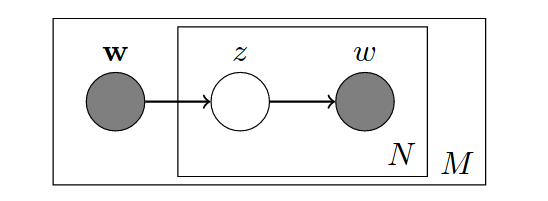
\includegraphics[width=0.6\textwidth, natwidth=548,natheight=201]{figs/PLSI_plate_notation.png}
\caption{Plate notation representing the PLSI model. \textbf{w} is the document index, $z$ is the topic drawn for the word $w$ from the topic distribution of the document}
\end{figure}
\end{center}
The result from PLSI is that every document is represented as mixing proportions
for the topics, given by $p(z|$\textbf{w}$)$. Even though PLSI is generative for 
the analyzed corpus, it is not generative for new documents, which means is that
there is no clear way of assigning probability to a document that is not part
of the training data.\cite{blei2003latent} Another problem is that the number 
of parameters in the model grows linearly with the number of documents.


\subsubsection{Latent Dirichlet Allocation (LDA)}

LDA is a topic model that was first presented as a graphical model for topic
discovery by David Blei, Andrew Ng, and Michael I. Jordan in 2003. The basic
idea is that documents exhibit multiple topics. LDA is a generative statistical
model that allows sets of observations to be explained by unobserved groups
that explain why some parts of the data are similar. For example, if
observations are words collected into documents, it posits that each document
is a mixture of a small number of topics and that each word's occurrence is
attributable to one of the document's topics.\cite{Blei:2012:PTM:2133806.2133826}

This is similar to PLSI, except
that in LDA the topic distribution is assumed to have a Dirichlet prior. 
In practice, this results in more reasonable mixtures of topics in a
document. The reduced document description result in PLSI is a vector where
each element describes the mixing proportion for a topic. A limitation with
PLSI is that there is no generative model for these proportions, making it
difficult to handle unseen documents. The Latent Dirichlet Allocation model
tries to solve this limitation by setting a Dirichlet prior on the topic
distribution.\cite{blei2003latent}
 
Suppose that we have a collection of documents, and we want to find an
organization for these, i.e. we want to do unsupervised learning. A common way
to do unsupervised learning is to assume that the data were generated by some
probabilistic process, and then to infer the parameters of this process. The
generative process is a specification of a parametrized family of
distributions. Learning is based on the principle of maximum likelihood, or
some refinement of this principle such as maximum a posterior probability.
 
The basic idea in LDA is that we define a topic to be a Dirichlet distribution
over a fixed vocabulary. Technically, the model assumes that the topics are
generated first, before the documents.\cite{Blei11introductionto} Now for 
each document in the collection, we generate the words in a two-stage process:

\begin{algorithm}[H]
\SetAlgoNoLine
1. Randomly choose a distribution over topics.

2. 
\For{each word in the document}{
	(a) Randomly choose a topic from the distribution over topics in 
	step 1
	
	(b) Randomly choose a word from the corresponding distribution over 
	the vocabulary
}
\end{algorithm}

This statistical model reflects the intuition that documents exhibit multiple
topics. Each document exhibits the topics with different proportion (step 1);
each word in each document is drawn from one of the topics (step 2b), where the
selected topic is chosen from the per-document distribution over topics (step
2a). All the documents in the corpus share the same set of topics, but each
document exhibits those topics with different proportion - that’s the
distinguishing characteristic of LDA. A more detailed explanation of the model
follows in section 2.2.3.1.

\paragraph{Model}

LDA is a probabilistic model of text documents, which assumes a collection of 
K topics. Each topic defines a multinomial distribution over the vocabulary 
and is assumed to have been drawn from a Dirichlet 
$\beta_k \sim Dirichlet(\eta)$.

In LDA, each document is represented by a mixture of the topics, with weight
$\theta_w^2$ for topic $z$ in document $w$. These weight have a Dirichlet prior,
parameterized by a hyper-parameter $\alpha$. Each topic is a probability
distribution over the vocabulary, with probability $\beta^w_z$ for word $w$ in
topic $z$. We define the following variables and notation:
\begin{itemize}
  \item[] $k$ is the number of topics.
  \item[] $V$ is the number of unique words in the vocabulary.
  \item[] $\theta$  is the topic distribution (of length $k$) for a document,
   drawn from a uniform Dirichlet distribution with parameter $\alpha$.
  \item[] $z_{n}$ is a topic assignment for $word w_{n}$, sampled from 
  $p(z_{n} = i|\theta) = \theta_{i}$.
  \item[] \textbf{w}$ = (w_{1}, ... , w_{N})$ is a document with $N$ words.
  \item[] $w_{n}^{i} = 1$ means that the word $w_{n}$ is the $i$-th word 
  of the vocabulary.
  \item[] $\beta$  is a $k \times V$ matrix, where each row $\beta_{i}$ 
  is the multinomial distribution for the $i$-th topic. That is, 
  $\beta_{ij} = p(w^{j} = 1 | z_{j} = i)$.
\end{itemize}

For each document $w$, in corpus $D$, the LDA generative process is as follows, 
with corresponding plate notation in Figure 2:

\begin{algorithm}[H]
\SetAlgoNoLine
1. Draw topic distribution $\theta_w \sim Dir(\alpha)$

2. 
\For{each of the $N$ words $w_n$}{
	(a) Draw a specific topic $z_n \sim Multinomial(\theta)$
	
	(b) Draw a word $w_n \sim Multinomial(\beta_{zn})$
}
\end{algorithm}

As seen in step 1, each document contains topics in different proportions,
determined by the scaling parameter $\alpha$. The individual words are drawn
from one of the $k$ topics in step (b), where the probability of each word
within a topic is parameterized by a $k \times V$ matrix , where $V$ is the
size of the specified vocabulary. The most probable words in each topic could
be used to identify the topic and gives an intuitive description for the topic.

We can see that this does in fact generate a document based on the topic 
mixture $\theta$, the topic-word assignments $z$, and the probability 
matrix $\beta$. Then, we can analyze a corpus of documents with LDA by 
examining $\beta$, which is the posterior distribution of topics, $\theta$ 
and $z$ conditioned on the documents. This reveals latent structure in
the collection that can be used for prediction or data exploration. 

Hence, we observe the document, and must infer the latent topic mixture 
$\theta$ and topic-word assignments $z$. LDA aims to infer:

\begin{equation}
p(\theta, \textbf{z} |\textbf{w}, \alpha, \beta)
\end{equation}

This
posterior can't be computed directly; it is usually approximated using Markov
Chain Monte Carlo (MCMC) or variational inference. Both methods are effective,
but also present significant computational challenges in large data sets
~\cite{onlineLDAvb}. In our implementation, we're using the online variational
LDA model, which is described in section 2.2.3.4.
 
The key difference in LDA compared to PLSI is that the process outlined above
actually is generative for documents. This means that, given a new document,
one can use the parameters learned previously to estimate the topic
distribution $\theta$ for this new document.
 
A limitation with the standard LDA model is the fix vocabulary. This means that
new words cannot enter the model and that you have to know a priori what words
will model the corpus effectively. A setting where this could be problematic is
when analyzing data where new words in the form of slang or names emerge over 
time. Another limitation is the fact that one has to state
the number of topics the model should use. This is not a big issue, but could
lead to some of the resulting topics to be insignificant.
\begin{center}
\begin{figure}[h]
\centering
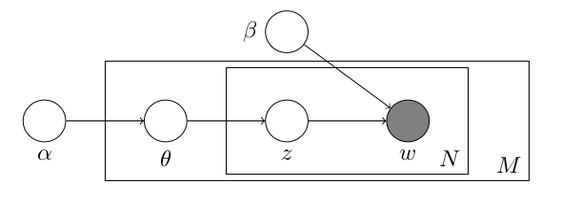
\includegraphics[width=0.6\textwidth, natwidth=561,natheight=197]{figs/LDA_standard_model.png}
\caption{Plate notation of the standard LDA model}
\end{figure}
\end{center}

\paragraph{Expectation Maximization}

The Expectation Maximization, or EM, algorithm is an approach to deriving an
algorithm for approximately obtaining maximum likelihood of variables in a
statistical model. Normally one obtains a maximum likelihood solution by taking
partial derivatives of the likelihood function with respect to all variables,
setting these derivatives to zero and solving the equations simultaneously.
\cite{Myung:2003}

Due to latent variables it is not always possible to solve the equations
directly and instead one typically gets two sets of equations that depend on
each other. The EM algorithm uses the idea that one could choose starting
values for the latent variables in the first set of equations, use the result
in the second set of equations, and then alternate between the two sets until
convergence.

The general idea behind the Expectation-Maximization algorithm is this:

\begin{enumerate}
\item Start with an initial estimate of what each parameter might be.
\item \textbf{E step}: Compute the likelihood that each parameter produces 
the data point.
\item Calculate weights for each data point based on the likelihood of it 
being produced by a parameter.
\item \textbf{M step}: Combine these weights together with the data to 
compute a better estimate for the parameters.
\item Repeat steps 2 to 4 until the parameter estimate converges.
\end{enumerate}


\paragraph{Variational Inference}

In LDA, our ultimate goal is to find the posterior distribution of latent topic variables after observing training data. However, computing this distribution is intractable, so we’re forced to approximate. One approximation approach is to 
use an optimization method called Variational Bayes. In the original paper it's 
being used a variational Bayes approximation of the posterior distribution;\cite{blei2003latent} alternative inference techniques use Gibbs sampling and
expectation propagation. The goal of variational inference is to approximate an
intractable probability distribution $p$, with a tractable one $q$, in a way
that makes them as close as possible given a similarity measure. In this thesis,
variational inference is used to approximate the posterior distribution of
latent variables. A new distribution over the hidden variables $q(z, \beta)$
(called the variational distribution) is  introduced. This new distribution has
properties such that it can be efficiently computed.\cite{Fox2011ATO}

In short, we approximate the true distribution by a simple distribution $q$, and associate parameters $\phi$, $\gamma$, $\lambda$ with the original parameters 
$z$, $\theta$, $\beta$ respectively. Recall that $z$ gives the topic assignments 
for each word in each document, $\theta$ gives the topic composition of each 
document, and $\beta$ gives the word-topic probabilities for each word and each 
topic. The variational distribution is a function of a set of free parameters that 
are optimized such that the variational distribution is as close as possible to 
the actual target posterior distribution where closeness is measured in terms of 
KL divergence.

Specifically, we have:
\begin{equation}
q(z_{di}=k) = \phi_{dw_{di}k}
\end{equation}
\begin{equation}
q(\theta_{d}) = dirichlet(\theta_{d}; \gamma_{d})
\end{equation}
\begin{equation}
q(\beta_{k}) = dirichlet(\beta_{k}; \lambda_{k})
\end{equation}

The posterior over the per-word topic assignments $z$ is parameterized by
$\phi$, the posterior over per-document topic weights $\theta$ is parameterized
by $\gamma$, and the posterior over the topics $\beta$ is parameterized by
$\lambda$. 

Our goal is to estimate $\phi$, $\gamma$ and $\lambda$. In both VB and 
online VB LDA, we alternate between two steps:
\begin{enumerate}
\item E-Step: Estimate $\phi$, $\gamma$ using the current value of $\lambda$
\item M-Step: Update $\lambda$, using the current value of $\phi$
\end{enumerate}

In Variational Bayes, we perform multiple passes over the entire dataset, 
checking each time for convergence. During each pass, the algorithm does an 
E-Step using the entire dataset and an M-Step, which updates $\lambda$ using 
$\phi$ values from every document. At a high level:

\begin{algorithm}
\SetAlgoNoLine
E Step:

\For{$d = 1$ to $numDocs$}{
	initialize $\gamma$
    
    \Repeat{change in $\phi < \epsilon$}{
        update $\phi$
        update $\gamma$
     }
}
M Step:

update $\lambda$
\end{algorithm}

The specific updates are:
\begin{equation}
\phi_{d,word_{i},k} \propto e^{E_{q}(log \theta_{d,k})+E_{q}(log\beta_{k,word_{i}})}
\end{equation}
\begin{equation}
\gamma_{d,k} = \alpha + \sum_{word_{i}}\phi_{d,word_{i},k}n_{d,word_{i}}
\end{equation}
\begin{equation}
\lambda_{k,word_{i}}=\eta +\sum_{d}n_{d,word_{i}}\phi_{d,word_{i},k}
\end{equation}
Where $n_{d,word_{i}}$ is the number of occurrences of $word_{i}$ in document $d$.
The algorithm above has constant memory requirements and empirically
converges faster than collapsed Gibbs sampling. However, it still requires a
full pass through the entire corpus in each iteration. It can be slow to apply
to very large datasets.

\paragraph{Online variational LDA}


An online variational inference algorithm is proposed by Hoffman et all.\cite{onlineLDAvb} for fitting $\lambda$, the parameters to the variational
posterior over the topic distributions $\beta$. The "online LDA" is nearly as
simple as the variational algorithm, but converges much faster for large
datasets. Variational inference requires to pass through the whole dataset for
each iteration, and that can be a problem when working with big datasets and is
not an option to use cases where the data is arriving constantly. The Online
Variational Inference algorithm aims to solve both problems without compromising
the quality of the obtained topics and with an algorithm nearly as simple as
Variational Inference. For this algorithm we will only highlight the differences
respect the Variational Inference and the resulting algorithm. The key
difference is the way to fit the variational parameter $\lambda$ respect the
Variational Inference explained in the previous section.

In short, we approximate the true distribution by a simple distribution $q$, and
associate parameters $\phi,\gamma,\lambda$ with the original parameters $z,\theta,
\beta$ respectively, as in VB. Recall that $z$ gives the topic assignments for each
word in each document, $\theta$ gives the topic composition of each document, 
and $\beta$ gives the word-topic probabilities for each word and each topic.

Our goal is to estimate $\phi, \gamma, \lambda$. In both variational 
and online variational LDA, we alternate between two steps:

\begin{enumerate}
\item E-Step: Estimate $\phi, \gamma$ using the current value of $\lambda$
\item M-Step: Update $\lambda$, using the current value of $\phi$
\end{enumerate}

In online Variational Bayes, we only make a single sweep of the entire dataset, analyzing a chunk of documents at a time. A chunk could be a single document, 
50 documents, or even the entire dataset. Let’s let a chunk be 1000 documents.

The online E-Step only uses the current chunk; instead of holding all the 
documents we now only have to hold 1000 in memory. The E-Step finds locally 
optimal values for $\phi$ and $\gamma$, while in the M-Step, we first compute 
$\lambda^{*}$, which is the value of $\lambda$ if we imagined that the entire 
dataset is made up of $\frac{numDocs}{chunkSize}$ copies of the current chunk. 
Then $\lambda$ is updated using a weighted sum of $\lambda^{*}$ and $\lambda$:

\begin{algorithm}
\SetAlgoNoLine
E Step:

initialize $\gamma$

\Repeat{change in $\phi < \epsilon$}{
        update $\phi$
        
        update $\gamma$
}
M Step:

compute $\lambda^{*}$

update $\lambda$
\end{algorithm}

We can see that unlike variational LDA, in online LDA we only need to hold a
small chunk of the data at a time, and once we’re done analyzing it, we never
need it again. As with batch, once we’ve estimated $\lambda$, we can find the 
most probable words for each topic by looking at the word probabilities in 
each row of $\lambda$.\footnote{\url{https://wellecks.wordpress.com/2014/10/26/ldaoverflow-with-online-lda/}}


\section{Related work}

\section{Methodology}

In this section, we explain the procedure that we followed in n order to apply the LDA model in our dataset. The dataset consists of two datasets: the one that contains all the information about EU projects founded for research and innovation under the FP4-H2020 and the dataset from USA about the awards/projects that got approved from 1994-2017. We consider the projects' description/abstract as the documents in LDA.
 

\subsection{EU dataset}

CORDIS (Community Research and Development Information Service) is the European Commission's primary public repository and portal to disseminate information on all EU-funded research projects and their results in the broadest sense. The website includes all public information held by the Commission (project factsheets, publishable reports and deliverables), editorial content to support communication and exploitation (news, events, success stories, magazines) and comprehensive links to external sources such as open access publications and websites. CORDIS is managed by the Publications Office of the European Union, on behalf of the European Commission's research Directorates-General and Agencies. CORDIS content dates back to the origin of the service in 1990 and the website has been online since 1994.

Below, we provide the general topics of the EU projects as listed in the EU Open Data Portal \footnote{https://data.europa.eu/euodp/en/data}:
\begin{itemize}
\item Agriculture, Fisheries and Food
	\begin{description}
	\item Agriculture, Food safety, Maritime affairs and fisheries
	\end{description}
\item Business
	\begin{description}
	\item Competition, Enterprise, Single market, Trade
	\end{description}
\item Culture and Education
	\begin{description}
	\item Audiovisual and media, Culture, Education training and youth, Multiligualism
	\end{description}
\item Customs and Tax
	\begin{description}
	\item Customs, Taxation
	\end{description}
\item Development and Humanitarian aid
	\begin{description}
	\item Development and cooperation, Humanitarian aid and Civil protection, Human rights
	\end{description}
\item Economy and Finance
	\begin{description}
	\item Budget, Economic and monetary affairs, Fraud prevention
	\end{description}
\item Employment and Social affairs
\item Enlargement and Foreign affairs
\item Environment and Energy
	\begin{description}
	\item Climate action, Energy, Environment
	\end{description}
\item EU institutions
	\begin{description}
	\item Institutional affairs
	\end{description}
\item Health
	\begin{description}
	\item Health, Sport
	\end{description}
\item Justice and Citizens’ rights
	\begin{description}
	\item EU citizenship, Consumers, Justice and Home affairs
	\end{description}
\item Regions and Local development
	\begin{description}
	\item Regional policy
	\end{description}
\item Science and Technology
	\begin{description}
	\item Space, Digital Economy and Society, Research and Innovation
	\end{description}
\item Transport and Travel
\end{itemize}

The data that are provided by CORDIS (via the EU Open Data Portal) are open, free and can be used in research, applications, commercial or non-commercial purposes. The dataset that we chose for the following analysis contains information about all the projects funded by the European Union from 1994 to 2017. These projects got approved under the framework programme (FP4-H2020) for research and technological development. For each project it is provided information, such as: reference, acronym, dates, funding, programmes, participant countries, subjects and objectives.

In the provided dataset, the information is splitted into CSV files, based on the framework program that each project belongs. The frameworks from 1994 to 2020 are listed below:

\begin{itemize}
\item FP4: fourth framework programme (1994-1998)
\item FP5: fifth framework programme (1998–2002)
\item FP6: sixth framework programme (2002–2006)
\item FP7: seventh framework programme (2007–2013)
\item H2020: Horizon 2020 framework programme (2014-2020)
\end{itemize}

\subparagraph{Data preparation}

Data cleaning is absolutely crucial for generating a useful topic model. We implemented the following steps, which are common to most natural language processing methods, in order to obtain the final corpus for the analysis:

\begin{itemize}
\item Remove punctuation and numbers
\item Tokenize documents
\item Remove stopwords
\item Create a dictionary
\item Filter out the most frequent and some rare words of the dictionary
\end{itemize}

To obtain the collection of the documents, we consider as ‘documents’ in LDA the project objectives, which is an accurate description for the project. We also added the ‘title’ value of each project to the objectives-documents, to increase the probability of finding accurate topics. For the majority of the projects the ‘start date’ and ‘end date’ value was null, so we kept the splitting of the dataset per framework, in order to keep the correlation to the time. We followed the same format in the dataset of USA awards.

\begin{center}
\begin{tabular}{l*{6}{c}r}
Framework & Years & No of docs & No of unique tokens & No of words in the corpus \\
\hline
FP4 & 1994-1998 & 14567 & 7293 & 364263 \\
FP5 & 1998-2002 & 17202 & 15756 & 1617232 \\
FP6 & 2002-2006 & 10091 & 15521 & 1437607 \\
FP7 & 2007-2013 & 25607 & 26499 & 3789837 \\
H2020 & 2014-2017 & 9055 & 15835 & 1342882 \\
\end{tabular}
\end{center}

As stopwords, we used the list that is provided by the Gensim Python library\footnote{http://radimrehurek.com/gensim/} and we added following very common words in the existing dataset: 'data', 'based', 'new', 'project', 'university', 'student', 'students', 'research', 'study', 'program', 'development', 'study', 'studies', 'provide', 'use'. We also removed the rare words that appear less than 5 times in the collection. Finally, we obtained a smaller corpus per framework (see the table above)

In this section, we explain the procedure that we followed in n order to apply the LDA model in our dataset. The dataset consists of two datasets: the one that contains all the information about EU projects founded for research and innovation under the FP4-H2020 and the dataset from USA about the awards/projects that got approved from 1994-2017. We consider the projects' description/abstract as the documents in LDA.
 

\subsection{USA dataset}

The National Science Foundation (NSF) is a United States government agency that supports fundamental research and education in all the non-medical fields of science and engineering. Its medical counterpart is the National Institutes of Health. The NSF funds approximately 24\% of all federally supported basic research conducted by the United States' colleges and universities. In some fields, such as mathematics, computer science, economics, and the social sciences, the NSF is the major source of federal backing.
 
The NSF organizes its research and education support through seven directorates, each encompassing several disciplines:

\begin{itemize}
\item Biological Sciences
\begin{description}
\item Molecular, Cellular and Organismal biology, Environmental science
\end{description}
\item Computer and Information Science and Engineering
\begin{description}
\item Fundamental computer science, Computer and networking systems, 
Artificial Intelligence
\end{description}
\item Engineering
\begin{description}
\item Bioengineering, Environmental systems, Civil and Mechanical systems, 
Chemical and Transport systems, Electrical and Communications systems, Design
 and Manufacturing
\end{description}
\item Geosciences
\begin{description}
\item Geological, Atmospheric and Ocean sciences
\end{description}
\item Mathematical and Physical Sciences
\begin{description}
\item Mathematics, Astronomy, Physics, Chemistry and Materials science
\end{description}
\item Social, Behavioral and Economic Sciences
\begin{description}
\item Neuroscience, Management, Psychology, Sociology, Anthropology, 
Linguistics, Science of science policy and economics
\end{description}
\item Education and Human Resources
\begin{description}
\item Science, Technology, Engineering and mathematics education at every level
\end{description}
\end{itemize}

The data about the awards \footnote{https://www.nsf.gov/awardsearch/download.jsp} are open, free and can be used in research and applications. The dataset that we chose for the following analysis contains information about all the projects that got funded by the NSF from 1994 to 2017.
 
In the provided dataset, the information is splitted into XML files, separated per year, from 1994 - 2017. In order to keep the correlation to time and be able to compare the two datasets later, we splitted the projects based on the year they were initialized (see Table below).

\subparagraph{Data preparation}

Just like the EU dataset, we followed the same preprocessing steps to obtain the final corpus. As stopwords, we used the list that is provided by the Gensim Python library and we removed following very common words in the existing dataset: 'data', 'work', 'based', 'new', 'project', 'university', 'student', 'students', 'research', 'study', 'program', 'development', 'study', 'studies', 'provide', 'use', 'understanding', 'important', 'support', 'proposed'. We also removed the rare words that appear less than 5 times in the collection. Finally, we obtained a smaller corpus per framework (see Table below).

\begin{center}
\begin{tabular}{l*{6}{c}r}
Framework         & Years & No of docs & No of unique tokens & No of words in the corpus \\
\hline
FP4 & 1994-1997 & 36752 & 28038 & 4346604 \\
FP5 & 1998-2001 & 37674 & 30728 & 5166316 \\
FP6 & 2002-2006 & 54212 & 38476 & 8837298 \\
FP7 & 2007-2013 & 87341 & 48277 & 15673424 \\
H2020 & 2014-2017 & 35581 & 32268 & 7379219 \\
\end{tabular}
\end{center}

\subsection{Model inference}

Details about the implementation, system specs etc.


\section{Analysis and results}


\section{Conclusion}

\section{Future work}

\bibliography{references}{}
\bibliographystyle{plain}

\end{document}